%% laad alle packages en style-opties in:
\documentclass[11pt,a4paper,titlepage]{article}
\usepackage[utf8]{inputenc}
\usepackage[margin=2cm,headheight=13.6cm]{geometry}
\usepackage{color}
\usepackage{listings}
\usepackage{graphicx}
\usepackage{todonotes}
\usepackage{caption}
\usepackage{float}
\usepackage{titling}
\usepackage{pgfkeys}
\usepackage{wrapfig}
\usepackage{booktabs}
\usepackage{adjustbox}
\usepackage{pdflscape}
\usepackage{tabulary}
\usepackage{courier}
\usepackage{graphicx}
\usepackage{subcaption}
\usepackage{multirow}
\usepackage{enumitem}
\usepackage[ampersand]{easylist}
\usepackage{pdfpages}
\usepackage{amssymb}
\ListProperties(Hide=100, Hang=true, Progressive=3ex, Style*=-- ,
Style2*=$\bullet$ ,Style3*=$\circ$ ,Style4*=\tiny$\blacksquare$ )
% ...
%\uspackage{rotating}
\definecolor{mygreen}{RGB}{0,127,0}
\definecolor{mygray}{RGB}{100,100,100}
\definecolor{mymauve}{RGB}{100,32,255}
\definecolor{lgray}{RGB}{230,230,230}
\lstset{ %
  frame=none,
  backgroundcolor=\color{white},   % choose the background color; you must add \usepackage{color} or \usepackage{xcolor}
  basicstyle=\footnotesize\ttfamily,        % the size of the fonts that are used for the code
  breakatwhitespace=false,         % sets if automatic breaks should only happen at whitespace
  breaklines=true,                 % sets automatic line breaking
  captionpos=t,                    % sets the caption-position to bottom
  commentstyle=\color{mygreen},    % comment style
  deletekeywords={...},            % if you want to delete keywords from the given language
  escapeinside={\%*}{*)},          % if you want to add LaTeX within your code
  extendedchars=true,              % lets you use non-ASCII characters; for 8-bits encodings only, does not work with UTF-8
%  frame=single,                    % adds a frame around the code
  keepspaces=true,                 % keeps spaces in text, useful for keeping indentation of code (possibly needs columns=flexible)
  keywordstyle=\color{blue},       % keyword style
  language=,                 % the language of the code
  morekeywords={*,...},            % if you want to add more keywords to the set
  numbers=left,                    % where to put the line-numbers; possible values are (none, left, right)
  numbersep=5pt,                   % how far the line-numbers are from the code
  numberstyle=\tiny\color{mygray}, % the style that is used for the line-numbers
  rulecolor=\color{black},         % if not set, the frame-color may be changed on line-breaks within not-black text (e.g. comments (green here))
  showspaces=false,                % show spaces everywhere adding particular underscores; it overrides 'showstringspaces'
  showstringspaces=false,          % underline spaces within strings only
  showtabs=false,                  % show tabs within strings adding particular underscores
  stepnumber=1,                    % the step between two line-numbers. If it's 1, each line will be numbered
  stringstyle=\color{mymauve},     % string literal style
  tabsize=4,                       % sets default tabsize to 2 spaces
  aboveskip=3mm,
  belowskip=3mm,
}

\usepackage{fancyhdr}
\pagestyle{fancy}
\rhead{Delft University of Technology}
\usepackage{datetime}
\usepackage{moresize}

\newdateformat{monthyeardate}{%
  \monthname[\THEMONTH] \THEYEAR}

\newcommand{\rulebreak}{%
	\par%
	\vspace{0.9cm}%
    \noindent\rule{4cm}{0.4pt}%
    \vspace{1.2cm}%
    \par%
}

\newcommand{\coverpage}[1]{%
	\pagenumbering{roman}%
	\thispagestyle{empty}%
	\lhead{\textsc{Pattern Recognition - Team 27}}%
    \title{Pattern Recognition, Delft University of Technology}%
    \author{Jurriaan Govers BSc, 4163753 \\ Sebastiaan Joosten BSc, 4103513 \\ Stijn van der Smagt BSc, 4306686 }%
    \newgeometry{left=5cm,bottom=2cm,right=5cm,top=2cm}%
	\begin{center}\hspace{0pt}\vfill%
    \uppercase{Pattern Recognition\\
    Delft University of Technology}
	\rulebreak%
    {\Large\textbf{Final Assignment}}
    
    \vspace{0.5cm}
    {\HUGE\textbf{\textit{#1}}}
    
    \vspace{0.5cm}
	\theauthor%
	\par%
	\vspace{0.9cm}%
    \noindent\rule{4cm}{0.4pt}%
    \vspace{0.45cm}
    %\pagebreak
    %\tableofcontents%
	\rulebreak%
    \monthyeardate\today\par
    \hspace{0pt}
	\end{center}%
    \vfill
    \hspace{0pt}
	\pagebreak%
    \restoregeometry%
    \pagenumbering{arabic}%
}



% Custom arguments for /fig command
\pgfkeys{
 /fig/.is family, /fig,
 default/.style = 
  {scale = 1,
   angle = 0},
 scale/.estore in = \figScale,
 angle/.estore in = \figAngle
}
\newcommand{\fig}[2][]{%
	\pgfkeys{/fig, default, #1}%
	\begin{figure}[H]%
    \centering
    \includegraphics[angle=\figAngle,width=\figScale\textwidth]{#2}%
	\end{figure}%
}

\newcommand{\filename}[1]{%
	\texttt{#1}%
}

\newcommand{\vhdl}[1]{%
  \lstinputlisting[language=vhdl]{#1}
}

\newcommand*\paths[1]{\lstset{inputpath=#1}\graphicspath{#1}}



%% code for bibliography
\usepackage{biblatex}
\usepackage{hyperref}
\usepackage{setspace}
\addbibresource{bibr.bib}
\defbibheading{bibempty}{}
\hypersetup{hidelinks,colorlinks=false,breaklinks=true,urlcolor=ocre,bookmarksopen=false,pdftitle={Title},pdfauthor={Author}}
\renewbibmacro*{doi+eprint+url}{%
  \printfield{isbn}%
  \newunit\newblock
  \iftoggle{bbx:doi}
    {\printfield{doi}%
     \iffieldundef{doi}{}{\renewcommand*{\finentrypunct}{\relax}}}
    {}%
  \newunit\newblock
  \iftoggle{bbx:eprint}
    {\usebibmacro{eprint}%
     \iffieldundef{eprint}{}{\renewcommand*{\finentrypunct}{\relax}}}
    {}%
  \newunit\newblock
  \iftoggle{bbx:url}
    {\usebibmacro{url+urldate}%
     \iffieldundef{url}{}{\renewcommand*{\finentrypunct}{\relax}}}
    {}}
%% end code for bibliography

\begin{document}
  \coverpage{Classification of Hand-Written Digits}
  \pagebreak
  
  \section*{Executive Summary}
Samenvatting over report (weet niet of het er in moet?)

 \section{Introduction}
  \label{Intro}
  This report describes the design and performance of a Pattern Recognition algorithm that is able to classify images of hand-written digits on bank cheques. It considers two cases:
  \begin{itemize}
  	\item \textbf{Case 1: The system is trained only one time, and then used in the field.} This means a large amount of training data is available.
  	\item \textbf{Case 2: The system is trained for each batch of cheques.} This means only a small amount of training data is available.
  \end{itemize}
Although Case 2 provides significantly less data than Case 1 (and this definitely has to be taken into account during the design of the classification system) it is worthy to note that both cases call for a supervised learning approach. \\
The available data will be extracted from the NIST-list, a large dataset containing labelled hand-written digits from 0 to 9. These images will be processed in order to make it easier to handle them. The loading of the list and processing of the images it contains is done in a separate function, named \texttt{myrep.m}. This function is described in detail in section \ref{sec:ImPros}. Implementing the pre-processing in this way enables the inclusion of the image-processing part of the algorithm in a later benchmark test. It also enables the user to keep the pre-processing consistent across the two different cases if desired.\\
\noindent After the processing, two classifiers will be trained, one for each of the aforementioned cases. These classifiers will be stored as $w$, so that they too can be implemented in the benchmark test. The design of these classifiers is described in detail in section \ref{sec:ClasDes}. \\
Both classifiers will be evaluated using various error estimations. This way, some indication of their performance can be made before sending them to the client. \\
\noindent Finally, to simulate the evaluation by the client for both cases, the benchmark test will be conducted by calling \texttt{e = nist\_eval(myrep,w,n)}. The error $e$ this function returns should be less than 5\% for case 1 and less than 25\% for case 2. An overview of the handling of the data as described in this section can be seen in figure \ref{fig:process_flow}.
\begin{figure}[H]
	\centering
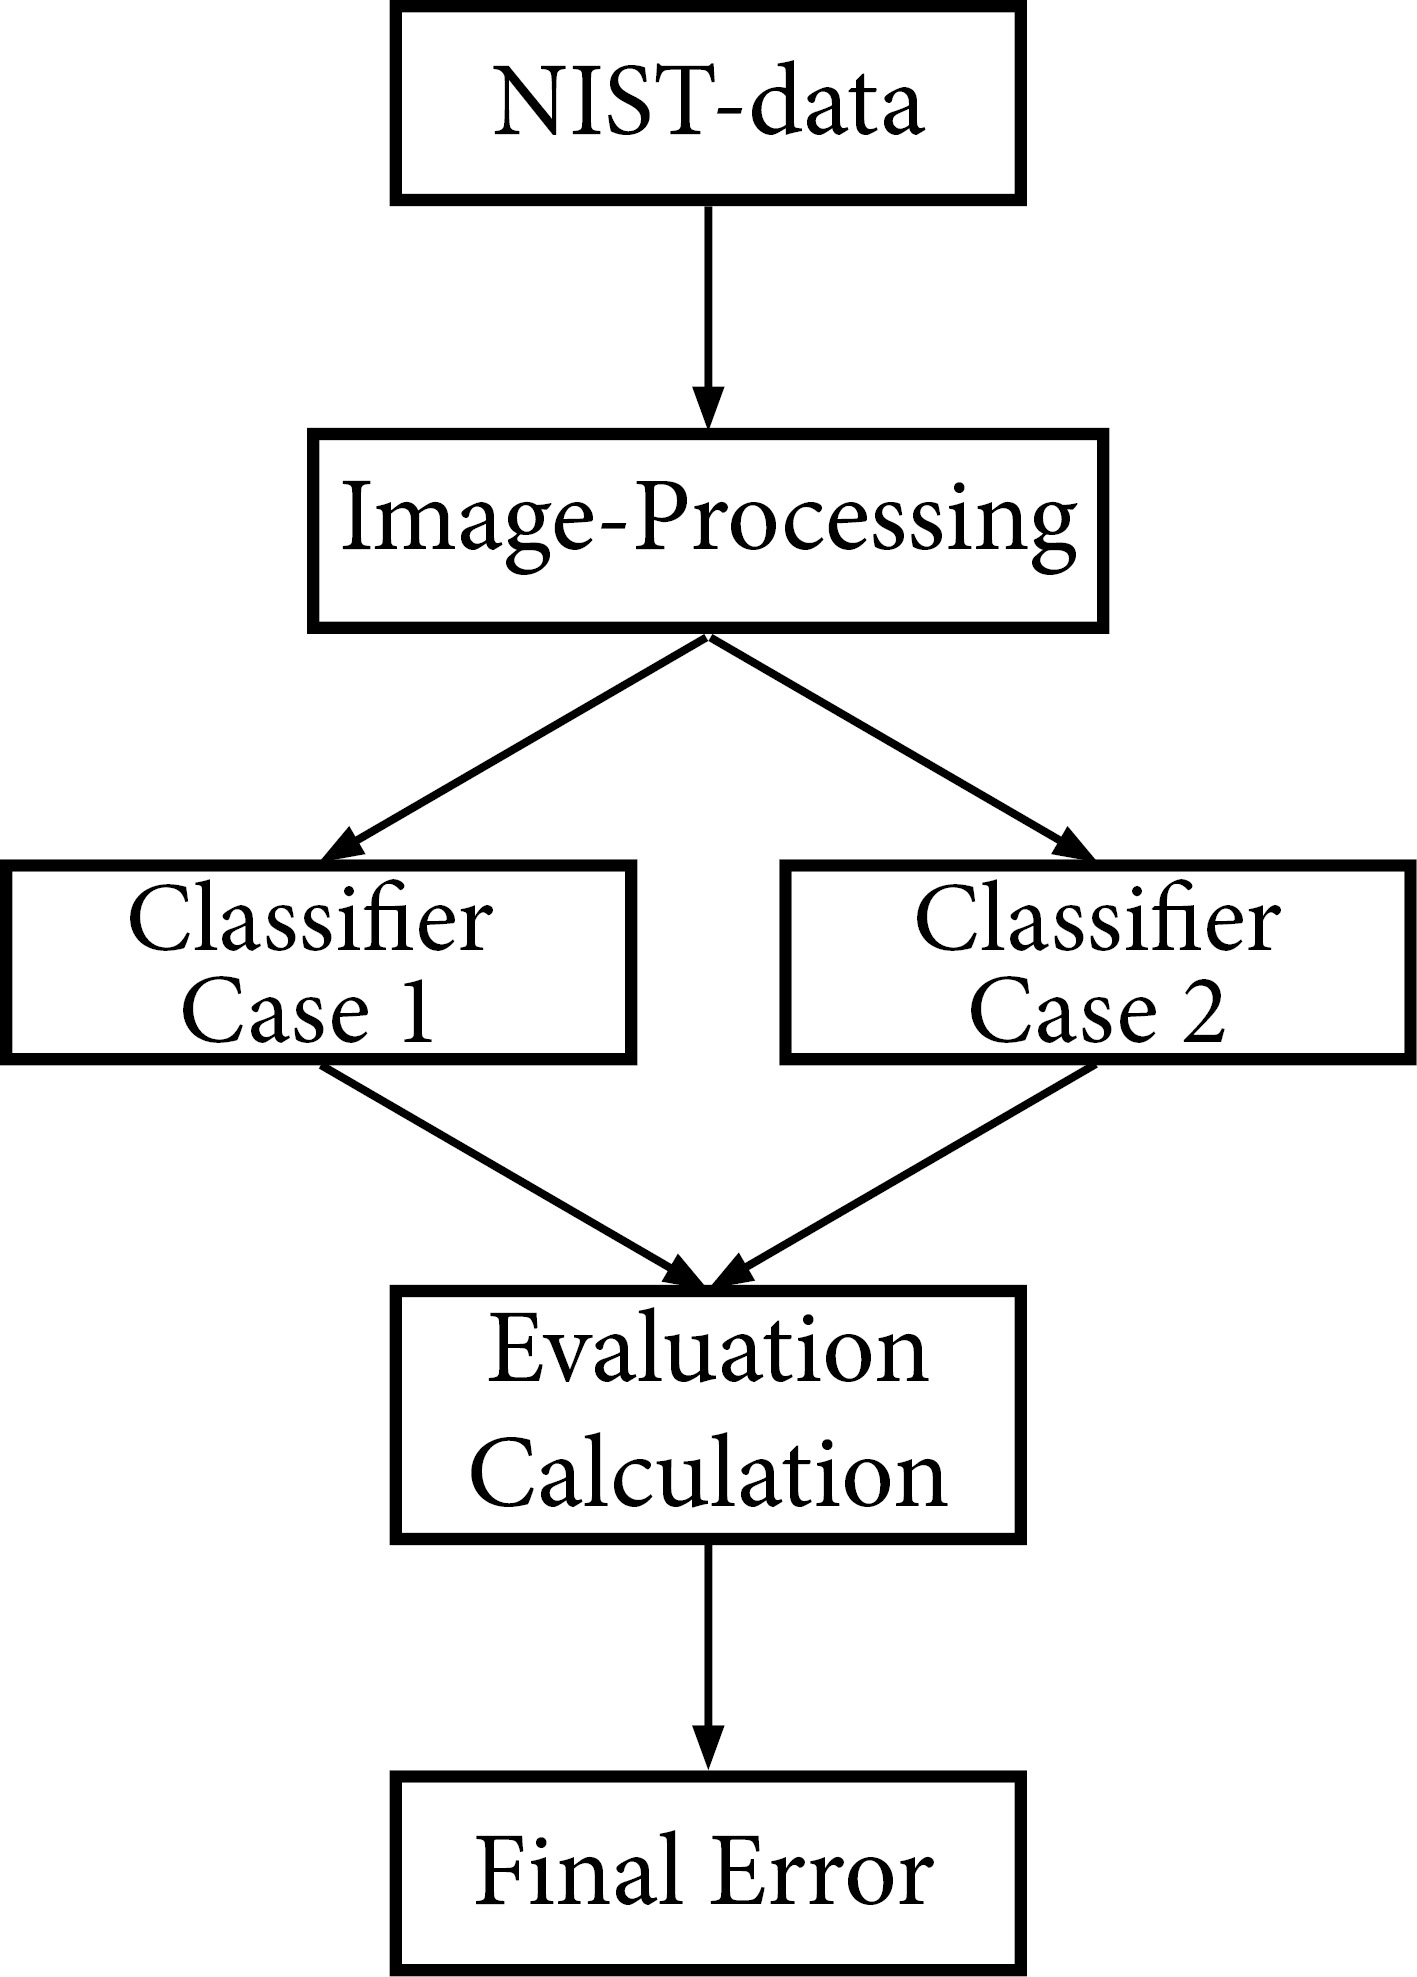
\includegraphics[scale=0.65]{images/Process_Flow.jpg}
\caption{Process of classification of the NIST-data for the two cases.}
\label{fig:process_flow}
\end{figure}
 
  




\end{document}